\documentclass{article}

%\usepackage[spanish]{babel}
\usepackage[utf8]{inputenc}
\usepackage{graphicx}

\title{Ecuaciones en diferencias}

\author{Ceci Alanís}

\date{Lunes, 18 de septiembre del 2017}

\begin{document}

\maketitle

\section{Ecuaciones de primer grado}

\subsection{Ecuaciones Lineales}

Una ecuacion lineal en diferencias de primer grado, tiene la forma $x_{n+1}=ax_n$ donde $a$ es una constante.  

La formula para resolver ecuaciones lineales es:
\begin{equation}
  \label{eq:2}
x_n=a^nx_0
\end{equation}

Por ejemplo, si iniciamos una inversion de 1000 pesos, con un interes mensual de 1\%, despues de 300 meses obtenemos los siguiente:

\begin{center}
  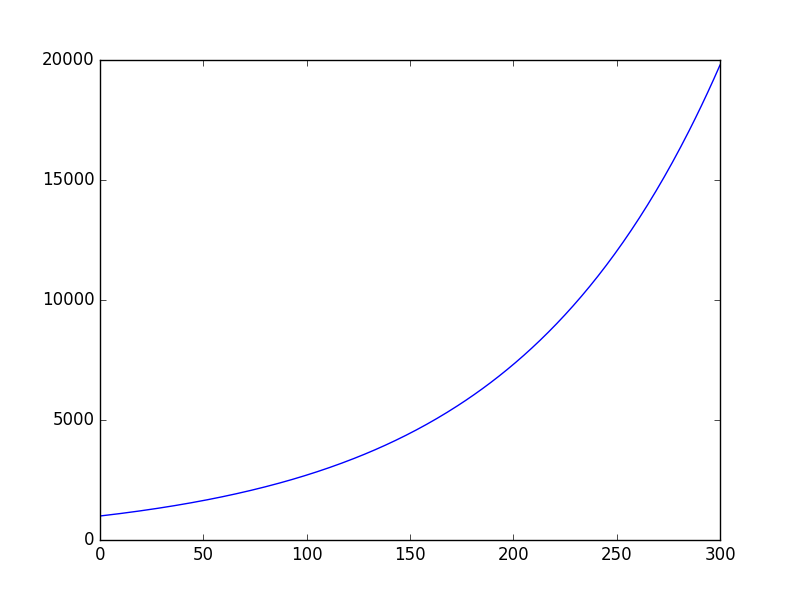
\includegraphics[width=8cm]{inversion.png}
\end{center}

\subsection{Ecuaciones Afines}

Una ecuacion afin en diferencias de primer grado, tiene la forma $x_{n+1}=ax_n+b $ donde $a$ es una constante.  

\begin{equation}
  \label{eq:1}
  x_n=a^n(x_0-\alpha)+ \alpha
\end{equation}

Donde $\alpha=\frac{b}{1-a}$.

Para deducir esta formula usamos $$\sum_{i=0}^{n-1}a^i= \frac{a^n-1}{a-1}$$.

\section{Ecuaciones de segundo grado}

El metodo para resolver estas ecuaciones esta inspirado en la formula \ref{eq:2}

\end{document}

